\section{Background}
\label{sec:background}

\subsection{GPU Address Translation}

Modern GPUs execute code in \emph{warps} of 32 lock-step
threads~\cite{aamodt_book,che_gpgpu_study,garland_cuda}, so a single memory
instruction can generate up to 32 virtual addresses at once. Coalescing~\cite{nyland_coalescing}
reduces this when threads share a page, but memory-intensive workloads with
large or strided access patterns routinely generate one or more unique VPNs
per warp instruction, creating translation pressure with no direct CPU
analog.

\begin{figure}[t]
  \centering
  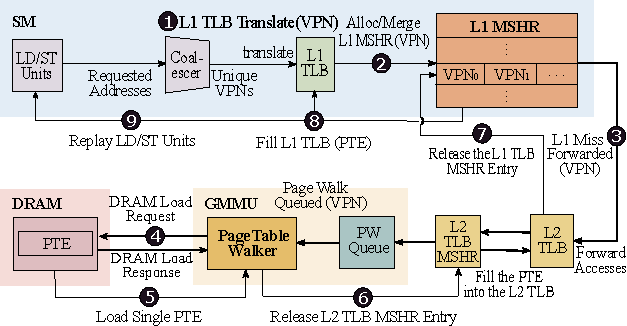
\includegraphics[width=\figwidth]{figs/fig02_TLB_diagram.pdf}
  \caption{GPU address translation hierarchy (SM86): L1 TLB per SM, shared L2 TLB,
  16 PTWs, and MSHR merging for same-VPN requests.}
  \label{fig:arch}
\end{figure}

Figure~\ref{fig:arch} shows the pipeline. Each SM hosts a private, fully-associative
32-entry L1 TLB~\cite{pichai_gpu_translation,translation_cpu}, flushed at kernel boundaries; on the
Ampere SM86 microarchitecture~\cite{nvidia_ampere} studied here, 46 SMs
operate independently. An L1 miss allocates an MSHR entry; a second request
for the same in-flight VPN merges into it rather than issuing a duplicate
walk, and both requestors unblock together on fill. Unmerged L1 misses
forward to the shared, chip-wide L2 TLB (1024 entries on SM86, servicing all
46 SMs), which performs the same same-VPN merge before dispatching to one
of 16 hardware page-table walkers (PTWs)~\cite{shin_irregular}, each
traversing the page table via sequential DRAM reads at hundreds to over a
thousand cycles. With 4\,KB pages, 1024 L2 entries give $4\,\text{MB}$ of
reach; footprints beyond that miss regardless of replacement policy.
Because only 16 PTWs exist, arriving misses queue behind occupied walkers,
and because the L2 MSHR merges by VPN, a single eviction that many warps
depend on stalls all of them at once when re-walked -- the mechanism
behind both the disproportionate cost of a dead-entry miss and the
disproportionate recovery from protecting one. This PTW bottleneck is the
primary reason TLB behavior dominates performance in translation-sensitive
GPU workloads~\cite{pichai_gpu_translation,avoiding_tlb,latpc}.

\subsection{Dead-Entry TLB Misses}

We define a \emph{dead-entry TLB miss} formally:

\begin{center}
\fbox{\begin{minipage}{0.92\columnwidth}
\smallskip
\emph{A TLB miss at virtual page $p$ at time $t$ is a \textbf{dead-entry miss} if $p$
was previously installed in the TLB, subsequently evicted before time $t$, and the
eviction preceded the miss without any intervening access to $p$ that would have
re-established a valid entry.}
\smallskip
\end{minipage}}
\end{center}

\noindent Equivalently, the page-table walker reconstructs a translation that was valid
and present within the current execution window, then discarded by LRU
replacement~\cite{lru,belady} -- the walk is logically redundant, not new
or stale. The classical three-C taxonomy~\cite{hill_smith_3c} describes
\emph{why} an eviction occurred; dead-entry is orthogonal, describing
\emph{what} the evicted entry was, and can arise from either a capacity
eviction (working set exceeds reach) or an interference-driven eviction (a
burst of other pages displaces a still-needed entry) -- the two root
causes behind the workload classes of Section~\ref{sec:characterization}.
Not every capacity or conflict eviction produces a dead-entry event: a
page never re-accessed within the execution window produces no re-walk.
This orthogonality is what makes dead-entry misses actionable where cold
and capacity misses are not: a cold miss needs prediction, a capacity miss
needs more reach, but a dead-entry miss is avoidable in principle simply
by remembering the recent eviction and protecting the re-installed entry
from immediate re-eviction -- the observation that motivates DEPOT.
